\section{Exponenciales y $e$.}

Como hemos insinuado antes, $e^x$ es una notación horrorosa que debería quedar exiliada de las explicaciones para principiantes. Es así que haremos un compromiso de olvidar su existencia hasta estar cualificados para usarla. Solicitamos que el lector descarte todo lo que sabe sobre exponentes hasta la educación secundaria.

Recopilando el poco entendimiento que parece consistente consigo mismo, $a^q$ solo tiene sentido cuando $a\in \mathbb{R}$ y $q \in \mathbb{Q}$ (uno puede cuestionarse la naturaleza de los números reales y qué significa multiplicar dos de ellos, pero queda fuera del alcance de este artículo). Cuando $q \in \mathbb{N}$, la potenciación se convierte en el conocido \enquote{multiplicar $a$ por sí mismo $q$ veces}. Sin embargo, tradicionalmente se introduce que, como $a^b a^c = a^{b + c}$ y como $\sqrt[2]{a} \cdot \sqrt[2]{a} = a$, es razonable decir que $a^{\frac{1}{2}}\cdot a^{\frac{1}{2}} = a^{\frac{1}{2} + \frac{1}{2}} = a$ y por ende que $a^{\frac{1}{2}} = \sqrt[2]{a}$. Extrapolando esto y usando propiedades similares, en general decimos que $a^{\frac{b}{c}} = \sqrt[c]{a^b}$.

Nótese que en ningún momento se ha mencionado la existencia de exponentes reales, y por un buen motivo: no tienen ningún sentido. ¿Cómo podría uno definir $e^x$ como una función continua si solo se permiten números racionales?

\subsection{El área bajo $\frac{1}{t}$.}

Tómese la función $f(t) = \frac{1}{t}$ y sea $A(x) = \int_1^x f(t) dt$ (Figura \ref{graph}). Uno puede imaginar esto como un plano con ejes $t$ e $y$ en el que se dibuja la función $f(t)$. Establecemos un punto fijo en $t = 1$ y dibujamos una línea vertical desde el eje $t$ hasta su intersección con $f(t)$. A su derecha, tenemos otro segmento vertical en $t = x$, también contenido entre el eje $t$ y la gráfica de la función. Uno puede imaginar a $x$ y su línea moviéndose libremente a lo largo del eje $t$, ensanchando y acortando la \enquote{ventana} entre los dos segmentos verticales. Con esto en mente, la función $A(x)$ describe el valor del área de esa ventana. Por supuesto, esto no es más que una integral.

\begin{figure}[H]
	\centering
	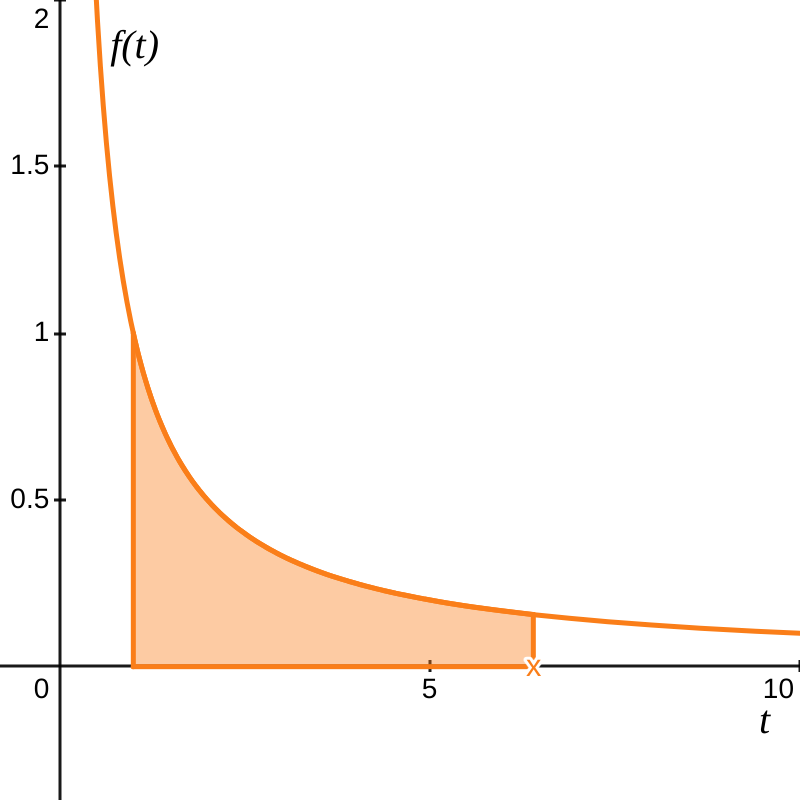
\includegraphics[width=\linewidth]{media/lnx.png}
	\caption{Representación gráfica de la integral de $1$ a $x$ de la función $f(t) = \frac{1}{t}$. La variable $x$ puede pensarse como un \enquote{control deslizante} que cambia cuán ancho es el marco de integración. Una gráfica interactiva está disponible en Desmos en \url{https://www.desmos.com/calculator/drhxhrnnr1}.}
	\label{graph}
\end{figure}

Nótese que lo que \enquote{varía} en $A(x)$ es $x$, en otras palabras, ese \enquote{control deslizante} que cambia cómo de ancha es nuestra ventana. $t$ no cambia con $x$, solo define a la función. Para esclarecer esto, uno puede considerar tomar valores específicos de $x$. Por ejemplo, $A(3) = \int_{1}^{3} f(t) dt$ significa \enquote{el área encerrada bajo la curva dibujada por $\frac{1}{t}$ entre $t = 1$ y $t = 3$}. Esto produce un número real con el valor $1.0986...$.

\textbf{Definimos} esa función de área como el \textit{logaritmo natural de $x$} (un nombre que por ahora puede perfectamente estar vacío de significado), escrito como $\ln(x) := A(x) = \int_{1}^{x} \frac{1}{t} dt$. Por el Teorema Fundamental del Cálculo, $A'(x) = (\ln(x))' = \frac{1}{x}$ (también puede ser demostrado por medio del Teorema del Sandwich). También definimos a $e$ como el número que satisface que $\ln(e) = 1$.

\newpage

\subsection{Propiedades de la función $\ln(x)$.}

Solo mirando al gráfico es inmediatamente obvio que para que la función $\ln(x)$ tenga sentido, $x$ debe ser mayor que $0$. Podemos analizar valores entre $0$ y $1$ invirtiendo los límites de integración y el signo del resultado. Es fácil ver entonces que $\ln(x)$ siempre es creciente, y que para valores entre 0 y 1, su valor es negativo. Además, en $x = 1$, su área queda colapsada hasta la nada, así que $\ln(1) = 0$.

Podemos demostrar las siguientes dos propiedades:

\begin{itemize}
	\item $\ln(ax) = \ln(a) + \ln(x)$ para todo $a, x \in \mathbb{R}^+$.
	\item $\ln(x^{\frac{p}{q}}) = \frac{p}{q} \ln(x)$ para todo $\frac{p}{q} \in \mathbb{Q}$ y $x \in \mathbb{R}^+$.
\end{itemize}

\subsubsection{Demostración de $\ln(ax) = \ln(a) + \ln(x)$.}

Empezamos tomando la derivada de $\ln(ax)$:

$$(\ln(ax))' = \frac{1}{ax} \cdot a = \frac{1}{x} = (\ln(x))'$$

Esto implica que

$$(\ln(ax) - \ln(x))' = 0$$

lo que quiere decir que

$$\ln(ax) - \ln(x) = c \textrm{ (constante)}$$

Para obtener el valor de $c$, podemos evaluar estas funciones en $x = 1$.

$$\ln(a) - \ln(1) = c \iff c = \ln(a)$$

Es decir

$$\ln(ax) = \ln(a) + \ln(x)$$

Este método también funciona para demostrar que $\ln(\frac{x}{a}) = \ln(x) - \ln(a)$. Nótese que esto funciona para \textit{todos los números reales positivos}.

\subsubsection{Demostración de $\ln(x^{\frac{p}{q}}) = \frac{p}{q} \ln(x)$}

Empezando de nuevo por su derivada,

$$\ln(x^{\frac{p}{q}})' = \frac{1}{x^{\frac{p}{q}}} \frac{p}{q} x^{\frac{p}{q} - 1} = \frac{p}{q} \frac{1}{x} = \frac{p}{q} (\ln(x))'$$

Otra vez, podemos restar la primera y la última derivada para obtener cero, implicando que $\ln(x^{\frac{p}{q}}) - \ln(x) = c$ con $c$ constante. En este caso, la constante resulta ser $c = 0$, dejando

$$\ln(x^{\frac{p}{q}}) = \frac{p}{q} \ln(x)$$

Esto es válido si $x > 0$ y si $\frac{p}{q} \in \mathbb{Q}$. Todavía no encontramos exponentes reales por ninguna parte.

\subsection{La función exponencial.}

Por estas propiedades, estamos autorizados a decir que:

$$\ln(e^2) = 2\ln(e) = 2$$
$$\ln(e^3) = 3\ln(e) = 3$$
$$\ln(e^4) = 4\ln(e) = 4$$
$$\ln(e^{q}) = q, \forall q \in \mathbb{Q}$$

Ahora definimos a la \textit{función exponencial} como el inverso de la función logaritmo natural: $\exp(x) := \ln^{-1}(x)$. Piénsese en el término \textit{exponencial} como un nombre en vez de un adjetivo. Por esta definición y por los resultados anteriores:

$$\exp(2) = \ln^{-1}(2) = e^2$$
$$\exp(3) = \ln^{-1}(3) = e^3$$
$$\exp(4) = \ln^{-1}(4) = e^4$$

En este sentido, se puede demostrar que la función $\exp(x)$ comparte bastantes similitudes con elevar $e$ a una potencia. Las propiedades habituales de los exponentes se traspasan también a esta función.

$$\exp(a + b) = \exp(a\cdot b)$$
$$\exp(a \cdot b) = \exp(a)^b$$
$$\exp\left(\frac{1}{2}\right) = \sqrt{e}$$
$$\exp(-1) = e^{-1}$$

Por esta bizarra correlación, es casi universal escribir $\exp(x)$ como $e^x$. Sin embargo, $\ln: (0, \infty) \to \mathbb{R}$, y por ende $\exp: \mathbb{R} \to (0, \infty)$. En otras palabras, podemos evaluar $\exp(x)$ en valores de $x$ irracionales. Esto no es un problema para la función $\exp(x)$, pero decir que $e^x$ puede tener una potencia irracional supone redefinir el mismísimo significado de \enquote{potencia}.

En esencia, definiremos toda potencia de exponente real en términos de $\ln$ y $\exp$. Aprovechando cierto abuso notacional, decimos que:

$$e^x := \exp(x)$$
$$a^x := \exp(x\cdot \ln(a)) = e^{x\cdot \ln(a)}$$

donde $a\in \mathbb{R}^+$ y $x\in \mathbb{R}$. Nótese que $-a^x \in \mathbb{R}$, mientras que $(-a)^x \in \mathbb{C}$. Esta es nuestra primera definición formal de $e$:

$$e := \exp(1) = \ln^{-1}(1) \iff \ln(e) = \int_{1}^{e} \frac{1}{t} dt = 1$$

\subsection{Otras definiciones de $e$.}

Como con muchas cosas en matemáticas, lo definido en una ocasión aparece en otros lugares inesperados. $e$ fue originalmente descubierto en el estudio de las tasas de interés en diferentes periodos de tiempo por Bernoulli.

$$\exp(x) = \lim_{n \to \infty} \left(1 + \frac{x}{n}\right)^n$$

$e$ es característico de aquéllos fenómenos en la naturaleza donde la tasa de cambio de una variable depende del valor de esa variable. Expresado usando ecuaciones diferenciales, $\exp(x)$ es la solución de:

\begin{equation}
	\begin{cases}
		f'(x) = f(x) \\
		f(0) = 1
	\end{cases}
\end{equation}

Si examinásemos $f$ mediante su expansión de Taylor, obtendríamos otra definición para la exponencial:

$$\exp(x) = \lim_{n \to \infty} \sum\limits_{k = 0}^{n} \frac{x^k}{k!}$$

\newpage
